% !TeX program = xelatex

\documentclass[12pt, a4paper]{article}

% Packages
\usepackage[inner=3.0cm, outer=3cm, top=2.5cm, bottom=2.5cm, includeheadfoot]{geometry}
\usepackage{graphicx}
\usepackage[spanish]{babel}
\usepackage{fancyhdr}
\usepackage{float}
\usepackage{setspace}
\usepackage{titlesec}
\usepackage[dvipsnames]{xcolor}
\usepackage[hidelinks]{hyperref}
\usepackage[utf8]{inputenc}
\usepackage{csquotes}  % Recomendado para biblatex
\usepackage[backend=biber,bibencoding=utf8,sorting=none]{biblatex} % Para bibliografía
\usepackage{listings}
%\usepackage{xcolor} % Para usar colores personalizados
\usepackage{caption}      % Para manejar captions
\usepackage{subcaption}   % Para las subfiguras
\usepackage{amsmath}
\usepackage{amssymb} 
\usepackage{comment}
\usepackage{appendix}
\usepackage{pdfpages}  % Paquete para insertar PDFs
\usepackage{xcolor} % Paquete básico para colorear tablas
\usepackage{array} % Para ajustar alineación de las columnas
\usepackage{cancel} % para cancelar valores en las ecuaciones


% Añadir archivo de bibliografía
\addbibresource{references.bib}

% Cambia el nombre del apéndice a "Apéndices"
\renewcommand{\appendixname}{Apéndices}
\renewcommand{\appendixtocname}{Apéndices}  % Cambia en el índice
\renewcommand{\appendixpagename}{Apéndices}  % Cambia en la página de título del apéndice
\renewcommand{\tablename}{Tabla}
\captionsetup[table]{name=Tabla} % Cambiar "Cuadro" por "Tabla"

% Header and Footer
\pagestyle{fancy}
\fancyhf{}
\fancyhead[L]{Generación de alta tensión}
\fancyfoot[L]{José Giménez Llanos - Álvaro Navarro Jorquera}
\fancyfoot[R]{\thepage}
\renewcommand{\footrulewidth}{0.4pt}
\setlength{\headheight}{14.5pt}

% Configuracion texto de código:
\lstset{
    language = Matlab,
  basicstyle=\ttfamily\footnotesize, % Si se quiere bastante mas pequeño sustituir \footnotesize por \scriptsize
  showspaces=false,           % No mostrar espacios con el símbolo ␣
  showstringspaces=false,     % No mostrar espacios en cadenas
  commentstyle=\color{green!60!black},
  keywordstyle=\color{blue},
  %stringstyle=\color{red},    % Color para las cadenas
  numberstyle=\tiny\color{blue},
  numbers=left,
  breaklines=true,
  frame=single,
  backgroundcolor=\color{gray!10},
  captionpos=b,
  caption=\lstname
}

\allowdisplaybreaks % Permite dividir alineaciones entre páginas

\begin{comment}



% Title Formatting
\titleformat{\section}{\normalfont\Large\bfseries}{\thesection}{1em}{}

% Cover Page
\title{
    \vspace{1cm} % Adjust vertical space
    %\includegraphics[width=0.55\textwidth]{MPOWER.jpg} \\ % Add your logo here (change "logo.png" to the actual filename)
    \begin{center}
        \begin{minipage}{0.3\textwidth}
            \includegraphics[width=\linewidth]{img/MPOWER.jpg} \\ % Logo 1
        \end{minipage}
        \hfill
        \begin{minipage}{0.3\textwidth}
            \includegraphics[width=\linewidth]{img/logo2.jpg} \\ % Logo 2
        \end{minipage}
        \hfill
        \begin{minipage}{0.3\textwidth}
            \includegraphics[width=\linewidth]{img/logo3.png} \\ % Logo 3
        \end{minipage}
    \end{center}
    \vspace{1cm} % Adjust vertical space after the logo
    \textbf{\Huge Diseño de una instalación fotovoltaica de utility scale} \\
    \vspace{1cm} % Adjust vertical space
    \large Energía Solar e Industria \\
    %\vspace{0.5cm} % Adjust vertical space
    %\large Date of Submission
}
\author{José Giménez Llanos}
\date{25/09/2024}
\end{comment}
\begin{document}

% Title Page
%\maketitle
\begin{titlepage}
    
    \newgeometry{ignoreall,top=2.5cm,bottom=1cm,outer=2.5cm,inner=2.5cm}
    \thispagestyle{empty}
    
    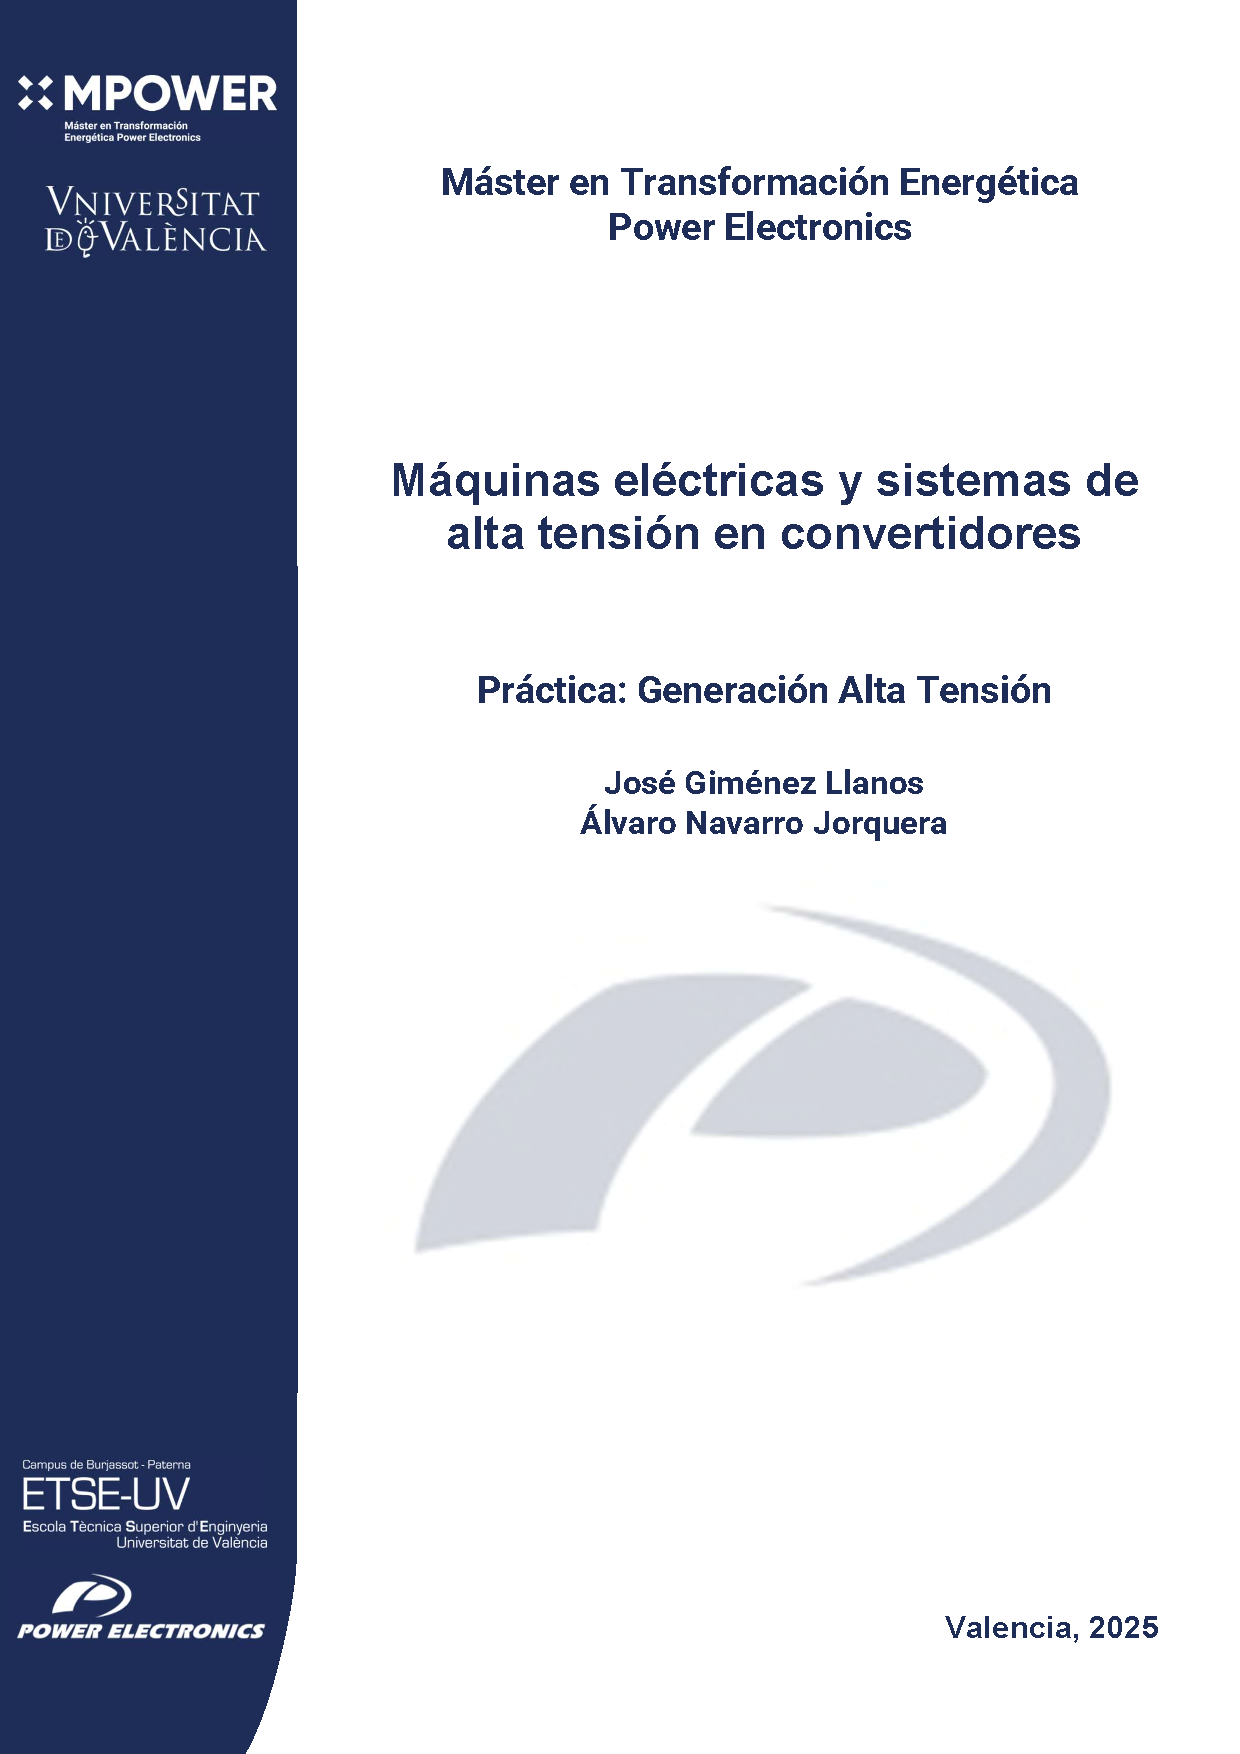
\includepdf[pages=-]{portada2.pdf}
    
\end{titlepage}
    
% A partir de aquí aplica los márgenes establecidos en configuracioninicial.tex
\restoregeometry
\thispagestyle{empty}
\newpage

% Table of Contents
\setcounter{page}{1}

\tableofcontents

\listoffigures
\newpage

\setlength{\parskip}{6mm}


\section{Introducción}
\section{Resolución}




\begin{comment}
    
% 4. Measurement/Testing Results
\section{Measurement}
Summarize the data gathered during the lab, including measurements and observations.
\begin{figure}[h!]
    \centering
    \includegraphics[width=0.8\textwidth]{example-image} % Example of adding a figure
    \caption{Test results for circuit 1}
    \label{fig:circuit1}
\end{figure}

% 5. Analysis and Discussion
\section{Analysis and Discussion}
Interpret the results obtained. Compare them with theoretical values, explain discrepancies, and discuss their significance.

% 6. Recommendations/Conclusions
\section{Conclusions}
Provide conclusions based on the results and discuss any recommendations for improvements, future work, or alternative solutions.
\end{comment}
%\newpage

%%%%%CUIDADO EN ESTE CASO ESPECIFICAMENTE HE QUERIDO PONER LAS REFERENCIAS DESPUES DE LOS ANEXOS PERO GENERALMENTE NO ES ASI
%\nocite{*} % Esto incluirá todas las referencias del archivo .bib
%\printbibliography[heading=bibintoc, title={Referencias}]

%\input{anexos}


% Bibliography
\newpage
\nocite{*} % Esto incluirá todas las referencias del archivo .bib
\printbibliography[heading=bibintoc, title={Referencias}]
\end{document}

